
\subsection{Identity-Transformation Algorithms}
\label{subsec:overview}

We design identity-transformation algorithms,
   %  $\mathcal{F}_{PID_{RP}}$, $\mathcal{F}_{PID_{U}}$ and $\mathcal{F}_{Acct}$,
    on an elliptic curve $\mathbb{E}$.
Table \ref{tbl:notations-protocol} lists the notations,
    and the subscript $j$ and/or the superscript $i$ may be omitted in the case of no ambiguity.

\begin{table}[tb]
\footnotesize
    \caption{The notations in the UPPRESSO protocols}
    \centering
%    \begin{tabular}{|c|c|c|}
    \begin{tabular}{|p{1.0cm}|p{6.60cm}|} \hline
    {\textbf{Notation}} & {\textbf{Description}} \\ \hline
    {$\mathbb{E}$, $G$, $n$} & {$\mathbb{E}$ is an elliptic curve over a finite field $\mathbb{F}_q$. $G$ is a base point (or generator) of $\mathbb{E}$, and the order of $G$ is a prime number $n$.} \\ \hline
    {$ID_U$} & {$ID_U = u \in [1, n)$, is the user's unique identity at the IdP; \textcolor{blue}{$u$ is kept unknown to RPs.}} \\ \hline
   {$ID_{RP_j}$} & {$ID_{RP} = [r]G$, is the $j$-th RP's unique identity; $r \in [1, n)$, \textcolor{blue}{is known to only the IdP.}} \\ \hline
    {$t$} & {$t \in [1, n)$, is a user-generated random integer in a login instance; \textcolor{blue}{$t$ is kept secret to the IdP.}} \\ \hline
    {$PID_{RP_j}^i$} & {$PID_{RP} = [t]{ID_{RP}} = [tr]G$; the $j$-th RP's pseudo-identity, in the user's $i$-th login instance to this RP.} \\ \hline
    {$PID_{U,j}^i$} & {$PID_U = [{ID_U}]{PID_{RP}} = [utr]G$; the user's pseudo-identity, in the user's $i$-th login instance to the $j$-th RP.} \\ \hline
     {$Acct_j$} & {$Acct = [t^{-1}\bmod n]PID_{U} = [ID_U]ID_{RP} = [ur]G$; the user's account at the $j$-th RP.} \\ \hline
    {$SK$, $PK$} & {The IdP's key pair, a private key and a public key, to sign and verify identity tokens and RP certificates.} \\ \hline
%    {$T$} & {The trapdoor to derive $Account$: $T=N_U^{-1} \bmod n$.} \\ \hline
    {$Enpt_{RP_j}$} & {The $j$-th RP's endpoint, to receive the identity tokens.} \\ \hline
    {$Cert_{RP_j}$} & {A signed RP certificate binding $ID_{RP_j}$ and $Enpt_{RP_j}$.} \\ \hline
%    {$PEnpt_{U,j}^i$} & {A user-generated random "pseudo-endpoint'', in the user's $i$-th login instance to the $j$-th RP.} \\ \hline
    \end{tabular}
    \label{tbl:notations-protocol}
\end{table}


For a user,
           a unique random integer $u$ is assigned by the IdP (i.e., $ID_U = u$).
When an RP is registering,
            the IdP generates a random number $r$, and $ID_{RP} = [r]G$, a unique point on $\mathbb{E}$, is assigned.
Here,
%$u, r \in [1,n)$, %$r$ is unknown to the RP, and
 $[r]G$ is the addition of $G$ on the curve $r$ times.

\vspace{0.5mm}
\noindent {\bf $\boldsymbol{ID_{\boldsymbol{RP}}}$-$\boldsymbol{PID_{\boldsymbol{RP}}}$ Transformation.} A user selects a random number $t$ ($1 \leq t <n$) as the trapdoor
         and calculates $PID_{RP}$.
\begin{equation}
PID_{RP} = \mathcal{F}_{PID_{RP}}(ID_{RP}) = [t]{ID_{RP}} = [tr]G
\label{equ:PIDRP}
\end{equation}
\noindent {\bf $\boldsymbol{ID_U}$-$\boldsymbol{PID_U}$ Transformation.}
On receiving an identity-token request with $ID_U$ and $PID_{RP}$,
    the IdP calculates $PID_{U}$.
\begin{equation}
PID_{U} = \mathcal{F}_{PID_U}(ID_U, PID_{RP}) =
  [{ID_U}]{PID_{RP}} = [utr]G
 \label{equ:PIDU}
\end{equation}


\noindent {\bf $\boldsymbol{PID_U}$-$\boldsymbol{Acct}$ Transformation.}
The trapdoor $t$ is sent to the target RP,
which checks that $PID_{RP}$ in identity tokens is equal to $[t]ID_{RP}$.
After verifying a token binding $PID_U$ and $PID_{RP}$,
    it calculates $Acct$ as below.
\begin{equation}
Acct = \mathcal{F}_{Acct}(PID_{U})
   = [t^{-1} \bmod n]PID_{U}
   \label{equ:Account}
\end{equation}

From Equations \ref{equ:PIDRP}, \ref{equ:PIDU} and \ref{equ:Account}, it is derived that
\begin{equation*}
   Acct =  [t^{-1}utr \bmod n]G = [ur]G = [ID_U]ID_{RP}
   \label{equ:AccountNotChanged}
\end{equation*}
The RP derives an \emph{identical permanent} account from the identity tokens in different login instances,
    with the help of $t$. %from the user.
Given a user, the accounts at different RPs are inherently unique;
while, given an RP, the accounts of different users are also unique.
It is impossible for the RP to derive $ID_U$ from either $PID_U$ or $Acct$ due to the elliptic curve discrete logarithm problem (ECDLP).
Because $t$ is random in $\mathbb{Z}_n$ and unknown to the IdP,
from the IdP's view,
    $PID_{RP}$ is indistinguishable from a random variable on $\mathbb{E}$,
    and the IdP learns nothing about $ID_{RP}$ from $PID_{RP}$.

Note that $r$ is kept secret to the RP; otherwise, two colluding RPs with $ID_{RP_j} = [r]G$ and $ID_{RP_{j'}} = [r']G$ could link a user's accounts by checking whether $[r']Acct_j = [r]Acct_{j'}$ or not.

\textcolor{blue}{A user generates $t$ and calculates $PID_{RP} = [t]ID_{RP}$.
After receiving $t$ from the user and extracting $PID_{RP}$ from an token,
    an RP checks that $PID_{RP} = [t]ID_{RP}$,
        because the correct account is derived only if this equation holds;
        otherwise, attacks happen as below.
To login as any $Acct$,
        a malicious user with $ID_{U'} = u'$ might generate a random number $t'$,
            and calculate $[t'u'^{-1}]Acct$ as $PID_{RP}$ to request an identity token.
Then, the IdP calculates $PID_{U'} = [u'][t'u'^{-1}]Acct = [t']Acct$.
Without checking $PID_{RP} = [t']ID_{RP}$ or not,
        the RP finally allows the malicious user to login as $[t'^{-1}]PID_{U'} = Acct$.}


\textcolor{blue}{On the contrary,
    if $t$ is generated and $PID_{RP}$ is calculated by the RP,
a user also needs to check that $PID_{RP} = [t]ID_{RP}$;
    otherwise, attacks happen as below.
A malicious user $U'$ initiates a login flow to an honest RP,
    and receives $PID_{RP}$.
Then it colludes with a malicious RP denoted as $RP'$,
    which sends $PID_{RP}$ to an honest user $U$.
Without checking $PID_{RP} = [t']ID_{RP'}$,
    this honest user will present a token binding $PID_U$ and $PID_{RP}$ to the malicious RP.
This token will enable $U'$ to login as the honest user's account at the honest RP.}
%In other words, this checking ensures RP designation,
%    because it is impossible to find $t$ and $t'$ satisfying that
%    $[t]ID_{RP} = [t']ID_{RP'}$,
%        when $ID_{RP} = [r]G$, $ID_{RP'} = [r']G$, but $r$ and $r'$ are unknown.
%See Section \ref{sec:analysis} for the detailed proofs of security and privacy.



\subsection{The Designs Specific for Web Applications}
\label{sec:web-design}
UPPRESSO works with commercial-off-the-shelf (COTS) browsers as the SSO user agent.
First of all, in UPPRESSO an IdP is not aware of visited RPs,
 so user agents (or browsers) have to deal with the forwarding of an identity token
    to the target RP, as well as the calculation of $PID_{RP}$.
On the contrary,
    in commonly-used SSO protocols \cite{OpenIDConnect,rfc6749,SAML,SAMLIdentifier} an IdP needs this information to ensure \emph{confidentiality} of identity tokens.
For instance, in the OIDC services, when an RP registers itself at the IdP, the \verb+redirect_uri+ parameter
    is set as its endpoint URL to receive tokens  \cite{OpenIDConnect}.
When the IdP is transmitting identity tokens to an RP,
    it utilizes HTTP 302 redirection with this endpoint as the target URL in HTTP responses,
     so a browser forwards it to the designated RP.

In UPPRESSO such user-agent functions are implemented by web scripts in COTS browsers,
and the scripts downloaded from an honest entity are also \emph{honest}.
%Section \ref{sec:discussion} discusses more efficient but less portable implementations with browser extensions.
Two scripts are from the visited RP and the IdP respectively,
    and each is responsible for the communications with the origin web server.
Only the RP script is not enough to implement a user agent;
    otherwise, the script will leak its origin to the IdP web server,
    because
    an HTTP request sent by the RP script
automatically carries an HTTP \verb+referer+ header that discloses the RP's domain.
Moreover, a trusted script from the honest IdP
ensures confidentiality of identity tokens (i.e., a token is sent to only the designated RP)
and interacts with users for attribute authorization,
    for the RP (and also the RP script) might be malicious.
Thus, on receiving an identity-token request,
    the IdP checks the \verb+referer+ header to ensure it is sent by the IdP script.

The RP script prepares $ID_{RP}$ and $Enpt_{RP}$ for the IdP script, through \emph{RP certificates}.
An RP certificate is signed by the IdP during the RP registration,
     binding the RP's identity and its endpoint. %(i.e., $ID_{RP}$ and $Enpt_{RP}$).
In a login instance
    the RP provides its certificate through the RP script, to the IdP script.
The IdP script %from the honest IdP,
    verifies the RP certificate to extract $ID_{RP}$ and $Enpt_{RP}$.
The IdP's public key is set in the IdP script, so
 a user does not configure anything locally,
    as it does in popular SSO systems \cite{OpenIDConnect, rfc6749, SAML,SAMLIdentifier}.

%Thus, to avoid the IdP server obtaining any evidence about the RP's identity and provide IdP's script with the RP certificate, the RP's script is also required to transmit the certificate to IdP script after it is downloaded from IdP server.

%A zero-knowledge proof may be designed,
%    the IdP script checks that the RP knows $t$ satisfying $PID_{RP} = [t]ID_{RP}$,
%    but knowing nothing about $t$ but only $PID_{RP}$.


After %calculating $PID_{RP}$ and
 receiving an identity token from the IdP,
    the IdP script needs to ensure the RP script will forward this token to $Enpt_{RP}$,
        which is bound along with $ID_{RP}$ in the RP certificate.
The scripts communicate with each other within the user browser through the \verb+postMessage+ HTML5 API,
%To avoid the honest user sending the identity token to an adversary,
and the receiver (i.e., the RP script)
 is restricted by the \verb+postMessage+ targetOrigin mechanism \cite{postm-targeto}:
when the IdP script sends messages,
 the receiver's origin is set as a parameter,
  e.g., \verb+postMessage(tkn, 'https://RP.com')+.
It consists of
    the protocol (i.e., \verb+https+),
    the domain  (i.e., \verb+RP.com+)
    and a port which may be implicit.
Only the script downloaded from this targetOrigin is a legitimate receiver.

%The \emph{RP certificates} deals with the problem of mapping an identity proof with its targeting RP.
%That is, the IdP script derives the RP's $ID_{RP}$ and origin from the RP certificate, while the $PID_{RP}$ is generated with this $ID_{RP}$. Thus, the IdP script always know the targeting RP of an identity proof, therefore, the \verb+postMessage+ mechanism can guarantee that the identity proof would not be sent to the adversary.

\textcolor{blue}{As mentioned above,
    a user needs to calculate (or check) $PID_{RP} = [t]ID_{RP}$,
    so this function should be implemented by \emph{honest} scripts.
Thus, $t$ is generated in the IdP script,
    and used to calculate $PID_{RP}$ with $ID_{RP}$ which is extracted from $Cert_{RP}$.
Since $ID_{RP} = [t^{-1}\bmod n]PID_{RP}$,
    this design relies on an honest IdP that does not steal $t$, $ID_{RP}$ or the RP's domain through malicious scripts,
        for any of them leaks the RP identity.
This leakage risk may be mitigated
    by implementing a user agent with browser extensions,
but users need to install the extension before visiting RPs.}

Finally,
    the browser downloads the RP script when visiting an RP,
     and this RP script opens a new window that downloads the IdP script.
We should prevent referer leakages when the IdP script is downloaded.
Generally, when a browser window visits another website not belonging to its opener's origin,
 the HTTP request to this website automatically carries a \verb+referer+ header (i.e., the opener's origin).
Such an HTTP header leaks the visited RP's domain to the IdP.
Fortunately, in UPPRESSO this newly-opened window is a \emph{redirection} from the RP to the IdP,
 but not a direct visit by browsers (Figure \ref{fig:process}, Steps 1.2-1.3).
This leakage is prevented by setting a \verb+referrer-policy=no-referrer+ header in the HTTP response from the RP,
 as it is redirected to the IdP.
So the HTTP request to download the IdP script carries no \verb+referer+ header.
This method is specified by W3C \cite{referer_policy} and widely supported.
We tested it in browsers such as Chrome, Safari, Edge, Opera and Firefox, and confirmed no referer leakage.




%in the SSO login flow,
 %   the user has to deal with RP endpoints (i.e., the URLs to receive identity tokens) by himself.
%In existing SSO protocols,
 %   an RP initially registers its endpoint at the IdP,
  %      and then in each login instance, the IdP will set this endpoint in the identity-token response.
%This instructs the user browser to forward it correctly;
  %  otherwise, confidentiality of identity tokens might be broken.
%In UPPRESSO the IdP is not aware of the visited RP and cannot set the endpoints,
 %       so \emph{RP certificates} are designed to instruct the user agents (or browsers) about
  %          the RP endpoint of an RP.
%An RP certificate is a document signed by the IdP during the RP initial registration,
  %   binding the RP's identity and its endpoint.
%This attribute certificate is sent by the RP in the login flow,
  %  so a user forwards identity tokens to the verified endpoint.









%However, in such system, the scripts is used to communicate between RP and IdP servers instead of HTTP URL redirection.
%The two scripts communicates with each other within the user browser through the standard \verb+postMessage+ HTML5 API.

%This mechanism can achieve the same security goal as the \verb+redirect_uri+ mechanism\cite{ChenPCTKT14} in OIDC systems.

%The RP script maintains the communications with the RP,
%    and it does not communicates directly with the IdP because an HTTP request launched by the RP script
%            will automatically carry an HTTP \verb+Referer+ header, which discloses the RP's domain.
%The IdP script downloaded from the IdP,
%    is responsible for the communications with the IdP,
%    and two scripts communicates with each other within the user browser through the standard \verb+postMessage+ HTML5 API.


\begin{figure*}[htb]
  \centering
  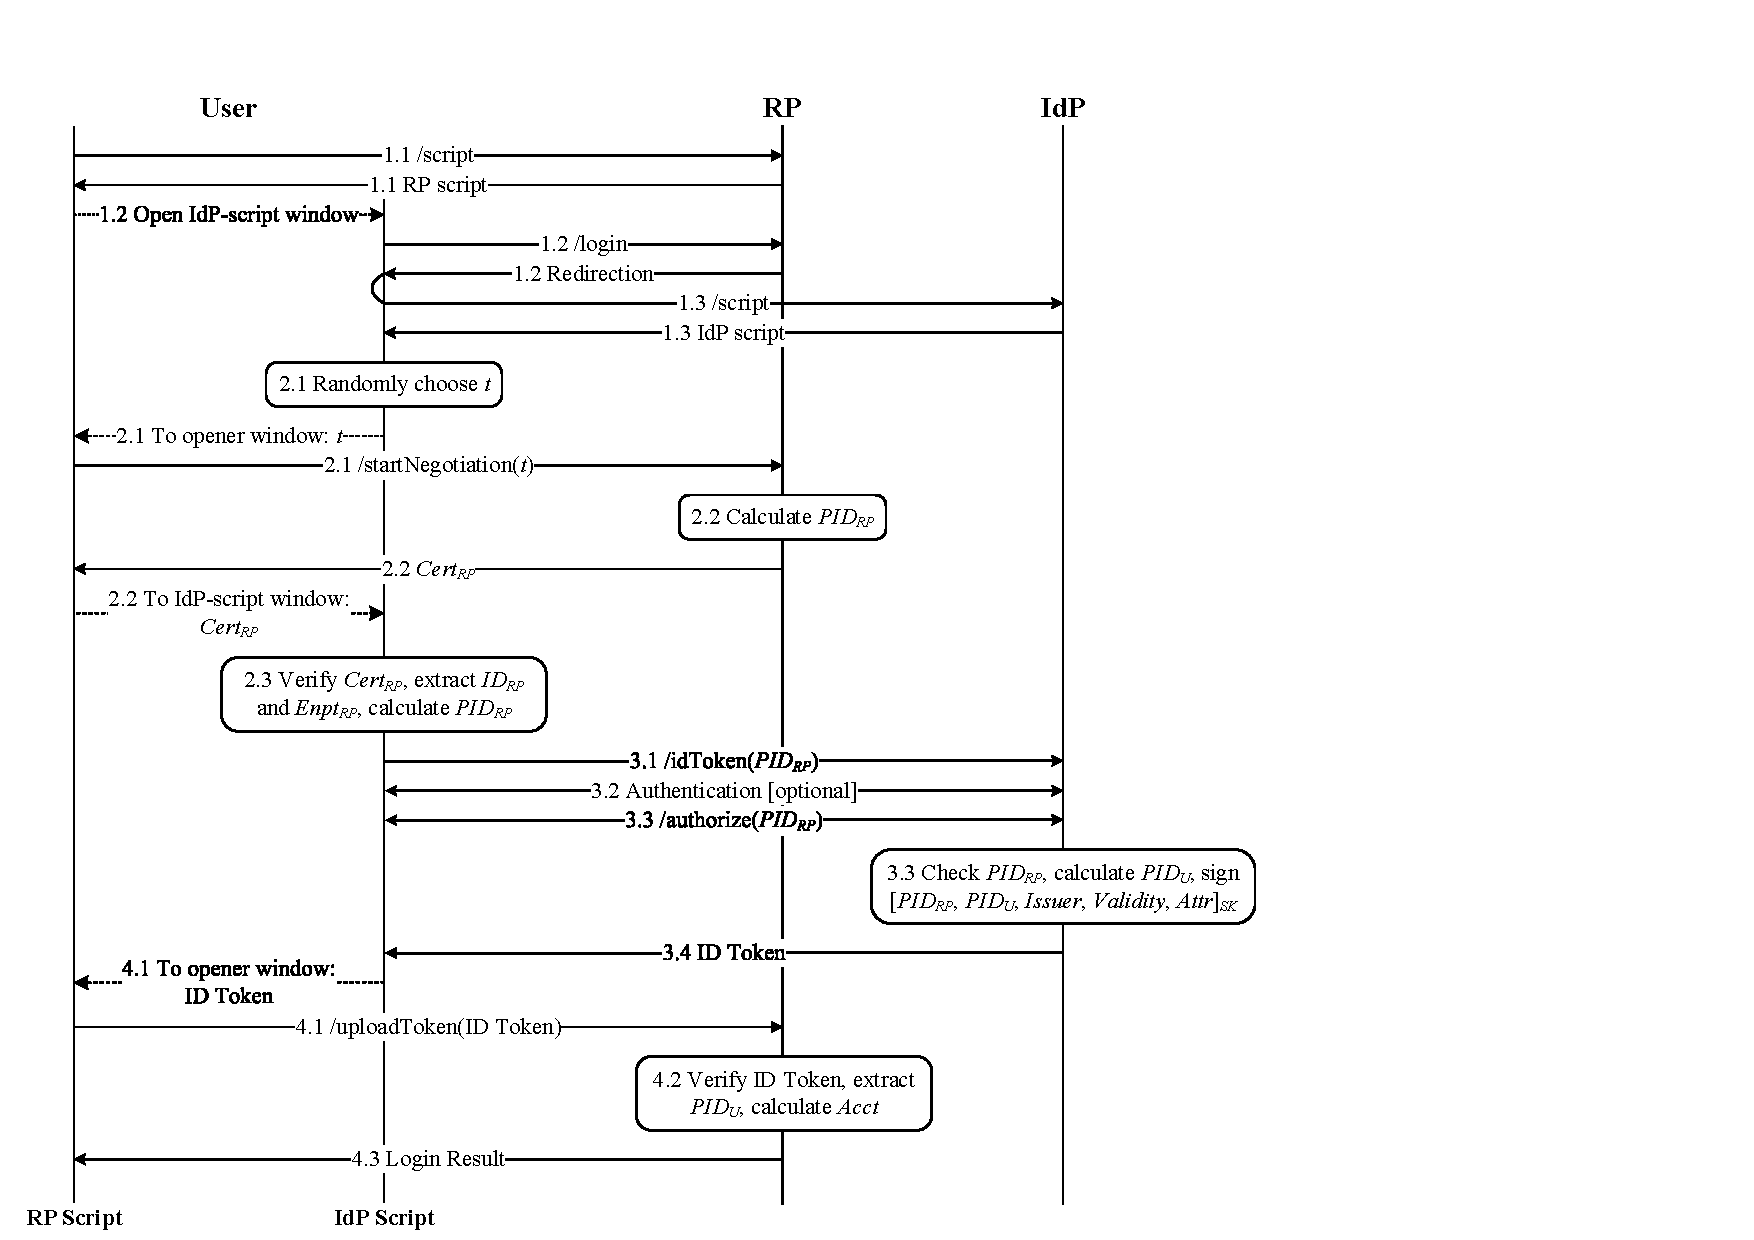
\includegraphics[height=0.575\textheight]{fig/process-js.pdf}
  \caption{The SSO login flow of UPPRESSO}
  \label{fig:process}
\end{figure*}



\subsection{The UPPRESSO Protocols}
\label{implementations}

\noindent \textbf{System Initialization.}
An IdP generates a key pair ($SK$, $PK$) to sign/verify identity tokens and RP certificates.
The IdP keeps $SK$ secret, and $PK$ is publicly known.


\vspace{1mm}
\noindent\textbf{RP Initial Registration.}
%Each RP launches an initial registration operation to finish configurations.
Each RP registers itself at the IdP to obtain $ID_{RP}$
 and its RP certificate $Cert_{RP}$ as follows:
\vspace{-\topsep}\begin{enumerate}
\setlength{\topsep}{0pt}
\setlength{\partopsep}{0pt}
\setlength{\itemsep}{0pt}
\setlength{\parsep}{0pt}
\setlength{\parskip}{0pt}
\item
An RP sends a registration request, including the endpoint to receive identity tokens
    and other information.
\item
The IdP randomly generates $r \in [1,n)$, until $ID_{RP} = [r]G$ is unique.
 %   but $r$ is kept unknown to the RP.
It signs $Cert_{RP} = [ID_{RP}, Enpt_{RP}, *]_{SK}$,
     where $[\cdot]_{SK}$ is a message signed using $SK$ and $*$ is supplementary information such as the RP's common name.
\item
The RP verifies $Cert_{RP}$ using $PK$,
    and accepts $ID_{RP}$ and $Cert_{RP}$ if they are valid.
\end{enumerate}

%Note that $ID_{RP}$ is generated by the IdP but not chosen by the RP;
%otherwise, a malicious RP might choose $ID_{RP}$ which reduces the difficulty to solve the ECDLP
%    (i.e., it is possible for the RP to derive $ID_U$ from $Acct = [ID_U]{ID_{RP}}$
%        or at least some information about $ID_U$).
%%%%%%%%%% 因为E上面的点,构成循环群、当n是素数的时候。所以,不会形成攻击。

%\vspace{0.5mm}
\noindent\textbf{User Registration.}
Each user registers once at the IdP to set up a unique random identity $ID_U = u \in [1, n)$ and the corresponding credential. $ID_U$ is kept unknown to RPs.
%This is similar to the steps in existing SSO systems.


\vspace{1mm}
\noindent\textbf{SSO Login.} A login instance %is typically launched through a browser,
%when a user attempts to visit an RP. It
consists of four steps, namely script downloading, RP identity transformation,
identity-token generation, and $Acct$ calculation, as shown in Figure \ref{fig:process}.
In this figure,
    the IdP's operations are linked by a vertical line,
        so are the RP's.
Two vertical lines split the user operations into two groups (i.e., in two browser windows),
    one of which is to communicate with the IdP,
                 and the other is with the target RP.
Each solid horizontal line means some messages between the user and the IdP (or the RP),
            and each dotted line means a \verb+postMessage+ invocation between two scripts (or browser windows) within the browser.

%In this figure, vertical bars stand for entity in the UPPRESSO system.
%At the user side, the vertical bars represent the browser's windows which are the containers of IdP and RP scripts.
%After a window is opened, the script in this window may change.
%For example, a window is opened at Step 1.2, and the script in this window belongs to the RP.
%However, after the redirection at Step 1.3, it visits the IdP server and downloads the script,
% so that the script inside this window changes into the IdP script.
%The main difference is that,
% the IdP script is only trusted by IdP server and allowed to communicate with IdP server.
% So does the RP script.

%%%, which calls three identifier-transformation functions following the login flow as shown in Figure \ref{fig:process}.
%%%Once a user attempts to login an RP, the SSO login is initiated.
%%%We use the OIDC implicit protocol flow as an example, to demonstrate  how to integrate the three functions $\mathcal{F}_{ID_{U} \mapsto PID_{U}}$, $\mathcal{F}_{ID_{RP} \mapsto PID_{RP}}$ and $\mathcal{F}_{PID_{U} \mapsto Account}$ into the typical SSO systems.

\vspace{0.5mm}
\noindent 1. {\em Script Downloading.}
The browser downloads scripts from the visited RP and the IdP.
\vspace{-\topsep}
\begin{itemize}
\setlength{\topsep}{0pt}
\setlength{\partopsep}{0pt}
\setlength{\itemsep}{0pt}
\setlength{\parsep}{0pt}
\setlength{\parskip}{0pt}
\item[1.1]
When attempting to visit any protected resources at the RP,
    the user downloads the RP script.
\item[1.2]
The RP script opens a window in the browser to visit the login path at the RP, which is then redirected to the IdP.
\item[1.3]
The redirection to the IdP downloads the IdP script.
\end{itemize}



%\vspace{1mm}
\noindent 2. {\em RP Identity Transformation.}
The user and the RP negotiate $PID_{RP} = [t]{ID_{RP}}$.
\vspace{-\topsep}
\begin{itemize}
\setlength{\topsep}{0pt}
\setlength{\partopsep}{0pt}
\setlength{\itemsep}{0pt}
\setlength{\parsep}{0pt}
\setlength{\parskip}{0pt}
\item[2.1] The IdP script locally chooses a random number $t$ in $\mathbb{Z}_n$,
 and sends it to the RP script through \verb+postMessage+.
The RP script forwards $t$ to the RP.
\item[2.2] On receiving $t$,
the RP verifies $1 \leq t < n$ and %calculates $PID_{RP}$.
%To acknowledge the negotiation of $PID_{RP}$, The RP
 replies with $Cert_{RP}$, which is then transmitted from the RP script to the IdP script,
    with the scope of requested user attributes.  % through \verb+postMessage+.
\item[2.3] The IdP script locally verifies $Cert_{RP}$, extracts $ID_{RP}$ and $Enpt_{RP}$ from $Cert_{RP}$, and calculates $PID_{RP}=[t]{ID_{RP}}$.
%It then creates a random endpoint $PEnpt_{U}$ for this login instance,
 %   to receive identity tokens from the IdP.
    % as the RP endpoint required by IdP.我们已经修改了协议,IdP并不require什么

\end{itemize}


%\vspace{1mm}
\noindent 3. {\em Identity-Token Generation.}
The IdP calculates $PID_U = [ID_U]{PID_{RP}}$ and signs an identity token. % The processes are as follows.
\vspace{-\topsep}
\begin{itemize}
\setlength{\topsep}{0pt}
\setlength{\partopsep}{0pt}
\setlength{\itemsep}{0pt}
\setlength{\parsep}{0pt}
\setlength{\parskip}{0pt}
\item[3.1]
The IdP script sends an identity-token request for $PID_{RP}$ on behalf of the user. %and the user attributes.
 %by checking whether this user is authenticated by IdP.

\item[3.2] The IdP authenticates the user, if not authenticated yet.

\item [3.3]
The IdP script obtains the user's authorization for each requested attribute,
    and sends the scope of authorized attributes. % to the IdP.
\textcolor{blue}{Then, the IdP %checks that the received $PID_{RP}$ is a point on $\mathbb{E}$,
    calculates $PID_U = [ID_U]{PID_{RP}}$, % for the user,
and signs $[PID_{RP}, PID_U, Issuer, Validity, Attr]_{SK}$,}
 where $Issuer$ is the IdP's identity, $Validity$ indicates the validity period, and $Attr$ contains the authorized user attributes.
\item[3.4] The IdP replies with the identity token, to the IdP script.
\end{itemize}

%\vspace{1mm}
\noindent 4. {\em $Acct$ Calculation.}
The RP receives the identity token and allows the user to login.
\vspace{-\topsep}
\begin{itemize}
\setlength{\topsep}{0pt}
\setlength{\partopsep}{0pt}
\setlength{\itemsep}{0pt}
\setlength{\parsep}{0pt}
\setlength{\parskip}{0pt}
\item [4.1]
The IdP script forwards the identity token to the RP script,
    which sends it to the RP through $Enpt_{RP}$.
\item[4.2] The RP verifies the identity token, including the IdP's signature and its validity period.
Then, \textcolor{blue}{the RP extracts $PID_U$ from the token, checks that it is equal to $[t]ID_{RP}$,}
and calculates $Acct = [t^{-1}]{PID_U}$.

\item [4.3] The RP allows the user to login as $Acct$.

\end{itemize}


If any verification or checking fails,
     this login flow will be halted immediately.
For example, the user halts it
    on an invalid $Cert_{RP}$.
\textcolor{blue}{The IdP rejects an identity-token request, if the received $PID_{RP}$ is not a point on $\mathbb{E}$.}
Or, the RP rejects an identity token
    if the signature is invalid or $PID_{RP}$ in it does not match the negotiated one.



\subsection{Compatibility with OIDC}
\label{subsec:compatible}
First of all, UPPRESSO and OIDC work with COTS browsers.
Among the four steps of the login flow in UPPRESSO,
    \emph{script downloading} prepares the user agent.
The user agent is responsible for the communications between the IdP and the RP,
    which are implemented by HTTP redirections in OIDC.
On the contrary, in UPPRESSO the scripts hide $Enpt_{RP}$ from the IdP
%in UPPRESSO
 %   when sending the identity-token request,
  %      the script replaces $Enpt_{RP}$ with $PEnpt_{U}$,
    and forward the identity token to $Enpt_{RP}$ extracted from the RP certificate,
%    that to protect the identity token from being sent to adversaries. 这句话与Compatibility无关
so the IdP does not set \verb+redirect_uri+ in the HTTP responses. % of identity tokens.
Most operations of \emph{RP identity transformation} are conducted within browsers,
 while the RP only receives $t$ to prepare an RP pseudo-identity
  and responds with  $Cert_{RP}$.
%The calculation of $PID_{RP}$ is viewed as the operation to prepare an RP identity in OIDC,
The static $Cert_{RP}$ is viewed as a supplementary message to users.
%The operations in the $PID_{RP}$ registration are almost identical to those in the RP Dynamic Registration of OIDC \cite{DynamicRegistration},
   % except that
   % in OIDC the IdP assigns the RP's identity  while in UPPRESSO this (pseudo-)identity is generated by the registered entity.
%Besides, the $PID_{RP}$ registration has a validity period.
Thus, compared with the original OIDC protocol, in these two steps, the IdP's operations are simplified
    and an RP customizes its \emph{dynamic} pseudo-identity.

The operations of \emph{identity-token generation} and \emph{$Acct$ calculation},
    are actually \emph{identical} to those of OIDC,
    because (\emph{a}) the calculation of $PID_U$ is viewed as a method to generate PPIDs
        and (\emph{b}) the calculation of $Acct$ is viewed as a mapping from the user identity in tokens
                    to an account at the RP.

Finally,
    this compatibility is experimentally confirmed by our prototype implementation:
     only 23 lines of Java code in MITREid Connect \cite{MITREid}, an open-source OIDC system,
 are modified
    to build an IdP of UPPRESSO (see Section \ref{subsec:proto-imple}).
%It will help the adoption and deployment of UPPRESSO.

%It follows a similar logic flow as OIDC in SSO login and only requires small modifications to perform identifier transformation.
%Here, we explain the modification in each of the five steps of its SSO login flow to show that UPPRESSO is compatible with OIDC, which indicates UPPRESSO can be easily integrated with other commonly used SSO systems.
%Among the five steps,
% the {\em scripts downloading} and {\em RP identifier transformation} steps are newly introduced by UPPRESSO.
%The browser is required to download two scripts from the IdP and RP and most of the designed operations in these two steps are performed by the scripts in the browser.
%So, we require minimal modifications to the IdP and RPs providing new network interfaces (i.e., the new URLs for downloading resources).
%The other three steps adopt a similar communication pattern as OIDC.
%In particular, the {\em $PID_{RP}$ registration} step can be viewed as a variant of the RP dynamic registration flow of OIDC \cite{DynamicRegistration}, which allows an entity to register its identity and endpoint at the IdP.

%UPPRESSO can also support the authorization code flow of OIDC with small modifications (to be discussed in Section \ref{sec:discussion}).


%Different from OIDC in which only RPs can call a dynamic registration, UPPRESSO allows any authenticated user to launch this process and register an RP identifier with the IdP.
%The {\em identity token generation} and {\em $Account$ calculation} steps adopt the same steps and functions as the implicit protocol flow of OIDC, while using a few different parameters. First, in identity token generation, $PID_U$ transformed from $ID_U$ is used to replace $ID_U$, which is directly supported by OIDC, similar as in the PPID approaches that also convert $ID_U$ into $PID_U$. The calculation of $Account$ from $PID_U$
%can be viewed as a customized step by the RP to derive its user account after the implicit protocol flow of OIDC ends.

%So,the identity token generation and $Account$ calculation steps of UPPRESSO can be viewed as a particular but compatible implementation of the implicit protocol flow of OIDC. It is worth noting that the identity token generation and $Account$ calculation steps of
%As shown in Figure \ref{fig:process}, in UPPRESSO, the SSO protocol for identity token is the same as in OIDC; the formats of identity token and corresponding request are the same as in OIDC; the correctness checks on the identity-token request at the IdP (i.e., consistency of RP' identifier and endpoint with the registered one) are the same as in OIDC; the correctness checks on the identity token (i.e., consistency of RP' identifier with the one in the request, integrity, validity time, freshness, and etc.) at the RP are the same as in OIDC.
%The above modifications could be completed automatically for each login, without affecting other communication pattern.

%以下为描述Step 2.3到7的详细内容.
%That is, the RP construct a request for identity token (Step 2.3); the user redirects this request to the IdP (Step 2.5); the IdP generates the identity token (Step 4), and sends it to the user (Step 5.1) who redirects it to the RP (Step 5.3); and finally the RP verifies the identity token (Step 6).

%However, UPPRESSO achieves privacy preservation by integrating  $\mathcal{F}_{ID_{U} \mapsto PID_{U}}$, $\mathcal{F}_{ID_{RP} \mapsto PID_{RP}}$ and $\mathcal{F}_{PID_{U} \mapsto Account}$, and  introduces the following modifications on OIDC.

%\begin{enumerate}
%  \item The identity token is bound with $PID_{RP}$ instead of $ID_{RP}$, which introduces the RP identifier transforming (Steps 1.2-1.5)  and $PID_{RP}$ registration (Steps 2.1-2.4).
%  \item The identity token is designated to one-time endpoint instead of RP's identifying endpoint, which requires the user to register the one-time endpoint in Step 2.1 and replace it with the original endpoint in Step 3.2.
%  \item IdP generates $PID_U$ based on ($PID_{RP}$, $ID_U$) instead of ($ID_{RP}$, $ID_U$).
%  \item The RP calculates $Account$ from the changing $PID_U$ instead of an unchanged one.
%\end{enumerate}

%上述modification如何实现的,简单描述
%to add: PID_{RP} transforming 和 RP identifer refreshing在user和RP的页面自己完成了。 都用现成的数据格式
%one-time endpoint 和endpoint
%The user automatically invokes the JavaScript functions to complete RP identifier transforming, one-time endpoint generating/replacing and $PID_{RP}$ registration for each login.
%While, the RP and IdP provide the corresponding web service to complete the processing automatically.

%The protocol of RP identifier transformation is based Diffie-Hellman key exchange \cite{DiffieH76}, while $N_U$ is provided to RP for computing the trapdoor and $N_{RP}$ is provided to the user for verifying the correctness of $Y_{RP}$.
